\documentclass{article}
\usepackage{graphicx}
\usepackage{caption}
\usepackage{subcaption}

    \begin{document}
\begin{figure}[htb]
    \centering
    \begin{subfigure}[b]{\textwidth}
        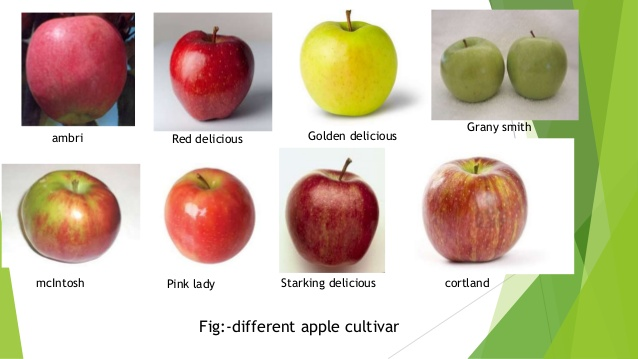
\includegraphics[width=0.6\textwidth]{images/apple_varieties.jpg}
        \subcaption{$Q^{*}$ values for arm 1}
        \label{fig:arm1}
    \end{subfigure}
%
    \begin{subfigure}[b]{\textwidth}
        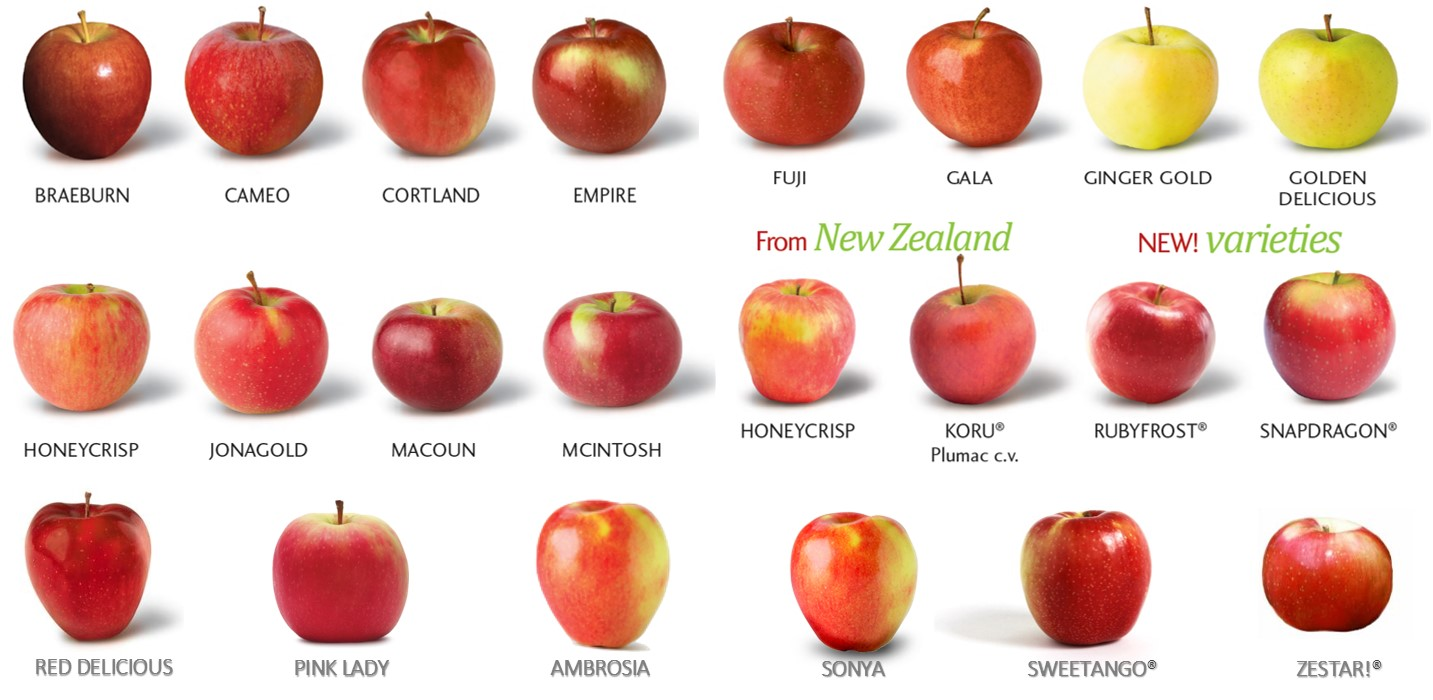
\includegraphics[width=0.6\textwidth]{images/apple_varieties2.jpg}
        \subcaption{$Q^{*}$ values for arm 2}
        \label{fig:arm2}
    \end{subfigure}
    \caption{$Q^{*}$ values for different arms}
\end{figure}
\begin{figure}[htb]\ContinuedFloat
    \centering
    \begin{subfigure}[b]{\textwidth}
        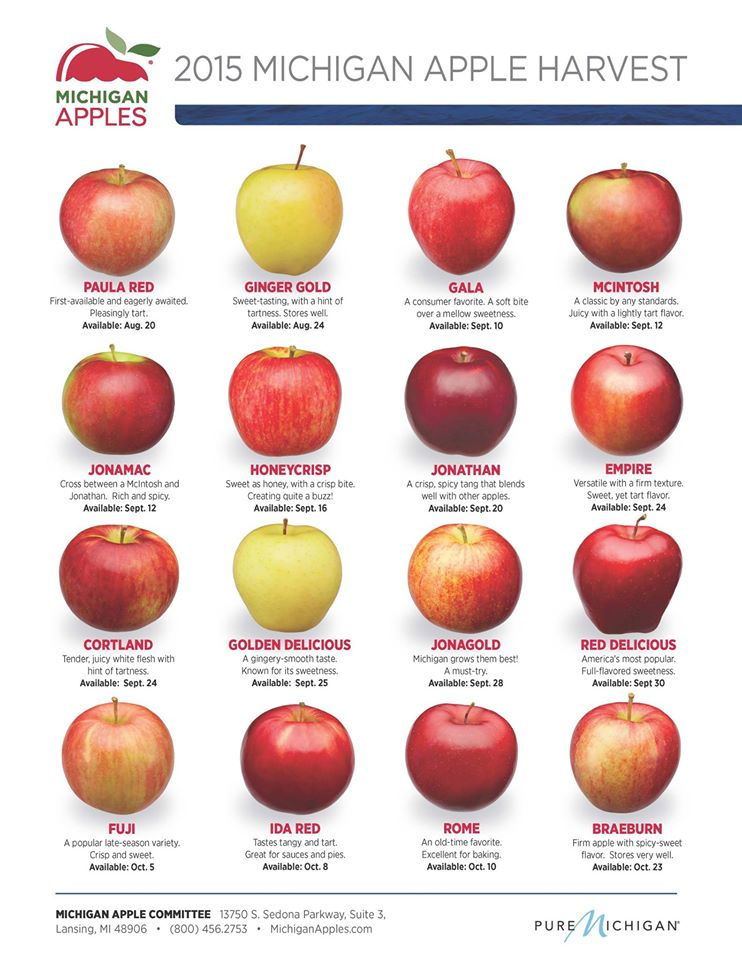
\includegraphics[width=0.6\textwidth]{images/apple_varieties4.jpg}
        \subcaption{$Q^{*}$ values for arm 3}
        \label{fig:arm3}
    \end{subfigure}
%
    \begin{subfigure}[b]{\textwidth}
        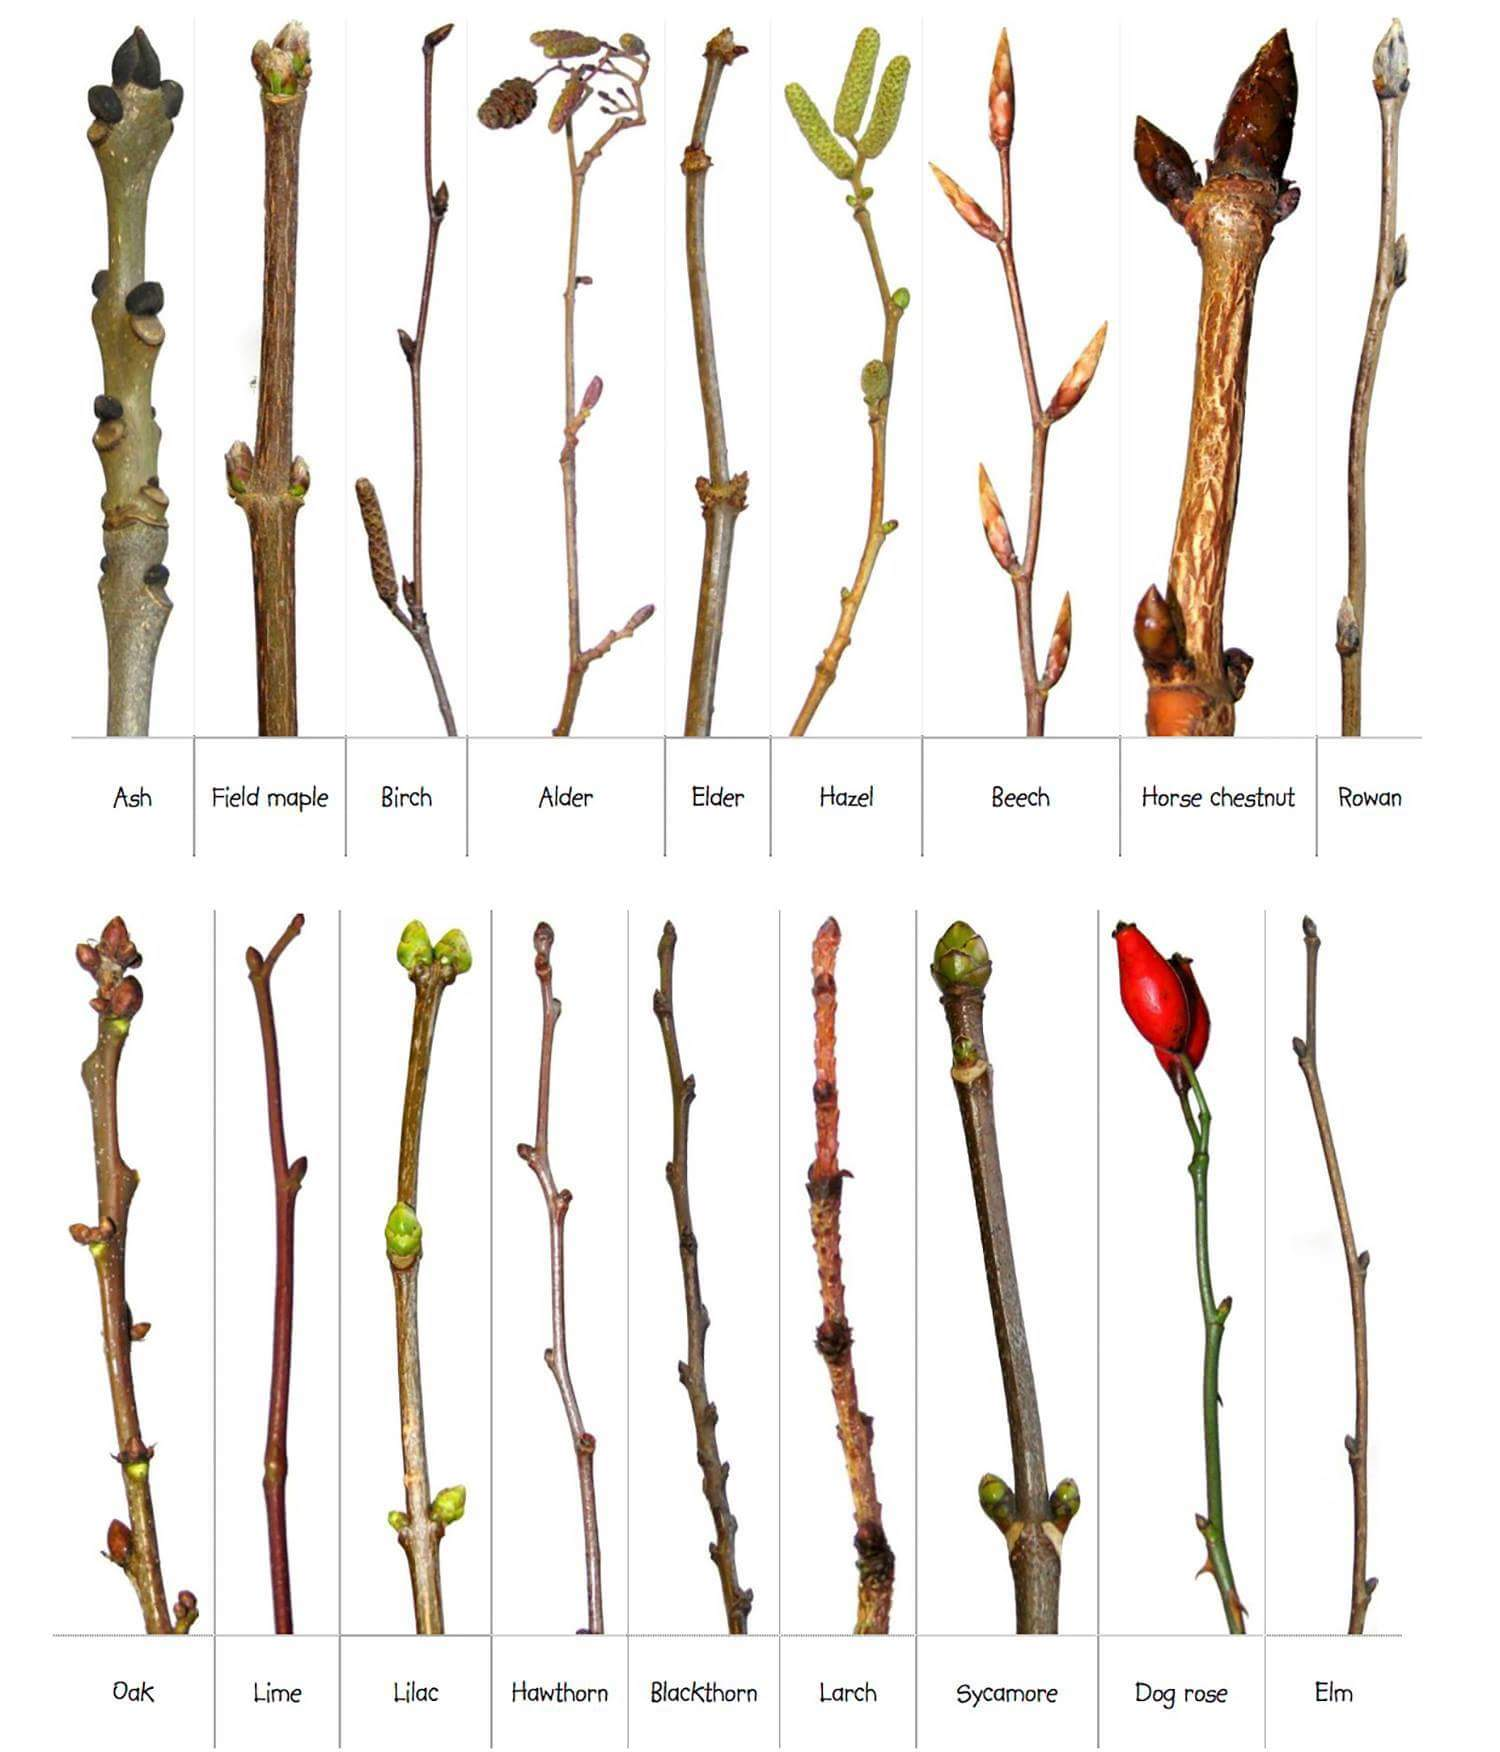
\includegraphics[width=0.6\textwidth]{images/Winter_twigs.jpg}
        \subcaption{$Q^{*}$ values for arm 4}
        \label{fig:arm4}
    \end{subfigure}
    \caption{$Q^{*}$ values for different arms (cont.)}
    \label{fig:arms}
\end{figure}
    \end{document}